\documentclass[11pt]{article}


\usepackage[utf8]{inputenc}
\usepackage[T1]{fontenc}
\usepackage[french]{babel}
\usepackage{newunicodechar}

\usepackage{graphicx}
\usepackage{fullpage}
\usepackage{times}
\usepackage{color}
\usepackage{needspace}
\usepackage{float}
\usepackage{listings}
\PassOptionsToPackage{hyphens}{url}
\usepackage{hyperref}
\usepackage{amsmath,amsfonts,amssymb,amsthm}
\usepackage{tabularx}
\usepackage{enumerate}

\begin{document}


\title{ \huge
  Implémentation de Go-Back-N et contrôle de congestion \\
  \Large Projet 1 de Réseaux I \\}

\author{Groupe 5\\DACHY Corentin (131563), JOSSE Thomas (171069)}

\date{Année Académique : 2017 - 2018\\
BAC 2 en Sciences Informatiques\\
\vspace{1cm}
Faculté des Sciences, Université de Mons}

\maketitle

\bigskip
\begin{center} \today \end{center}

\newpage

\section{Construction et exécution}
Pour compiler et exécuter notre application vous pouvez soit exécuter Ant en vous plaçant dans le dossier ou se trouve le fichier \textit{build.xml} et en lançant la commande \textbf{\textit{ant}} qui va compiler et lancer la démo directement. Soit lancer le fichier \textit{reso.examples.gobackn.Demo} dans le dossier build après avoir lancé \textbf{\textit{ant build}}. A la fin de vos tests vous verrez 2 nouveaux fichiers apparaître : "Plot.log" et "Status.log". Le fichier Plot.log contiendra les infos nécessaires à la création du plot tandis que le fichier Status.log contiendra tout ce qui s'est passé lors du test comme les pertes de paquets , les envois et réceptions de ceux-ci et les time-out.
\section{Structure de l'implémentation}

L'implémentation de Go-Back-N se présente comme l'attache de \bfseries GbnApplication \mdseries aux Host du Network, ce qui leurs permettra de communiquer entre eux. \\
Ces GbnApplication peuvent être de deux types (un à la fois, chaque type héritant de la classe abstraite GbnApplication): \bfseries GbnSender \mdseries  et \bfseries GbnReceiver\mdseries. Eux même possédant un \bfseries GbnProtocol\mdseries : respectivement un \bfseries GbnSendingProtocol \mdseries et un \bfseries GbnReceivingProtocol\mdseries .

\begin{figure}[h]
  \hfill\hbox to 0pt{\hss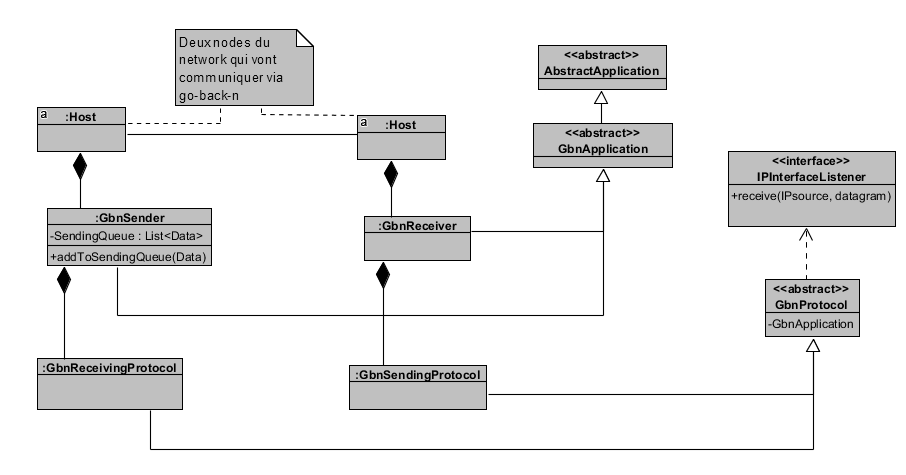
\includegraphics[scale=0.86]{bwuml.png}\hss}\hfill\null
  \caption{Diagramme de classe simplifié}
\end{figure}

C'est au niveau du GbnSender que l'on retrouve les informations à envoyer à un autre host (possédant un GbnReceiver). Dans notre implémentation, ces informations à envoyer se présentent comme une liste de String (notons cependant qu'il suffit de se tenir à la convention que les bytes sont représenté sous la forme de leurs caractère associé en ASCII et d'imposer une taille égale, 1 par exemple, à chaque String pour retrouver les datas à envoyer sous la forme d'un paquet de bytes). \\
Pour se faire, le GbnSender va laisser son GbnReceivingProtocol y accéder. Ce dernier, avec le GbnReceivingProtocol, comporte la véritable implémentation de Go-Back-N. Ces deux protocols vont s'envoyer des \bfseries GbnMessage \mdseries , des messages comportant un numéro de séquence. Plus précisément, le GbnSendingProtocol enverra des \bfseries DataMessage\mdseries , comportant également des informations à transmettre (un String ici) tandis que le GbnReceivingProtocol enverra des \bfseries ACK \mdseries (ACK et DataMessage sont deux classes héritant de la classe abstraite GbnMessage) .\\ 
\\
C'est donc dans le GbnSendingProtocol que nous retrouverons le pipelining et la gestion de congestion.


\section{Go-Back-N (pipelining)}
\subsection{La "Window"}
La "window" est une représentation (provenant du cours) de l'état actuel ainsi que des limites du pipelining. \\
Le GbnSendingProtocol comporte trois variable relative à la window, toute trois de type int: \\
-\bfseries nsq \mdseries : "next sequence number", le numéro du prochain packet à envoyer. Une fois la connection établie, nsq vaudra 0, car le prochain packet à envoyer sera le premier packet (numéro 0). Notons qu'nsq est initiallement initialisé à -1, car un paquet de numéro -1 ne contenant pas d'information autre que "je suis le paquet d'initialisation" sera envoyé avant de commencer l'envoi d'informations à proprement parlé \\
-\bfseries base \mdseries : Numéro du premier paquet dans la window. Autrement dit, base désigne le premier paquet dont la réception n'a pas encore été confirmée par un ACK \\
-\bfseries N \mdseries : La taille de la window, la limite du pipelining. Il ne sera pas possible d'envoyer un paquet de numéro de séquence superieur ou égal à base+N \\

\begin{figure}[h]
  \hfill\hbox to 0pt{\hss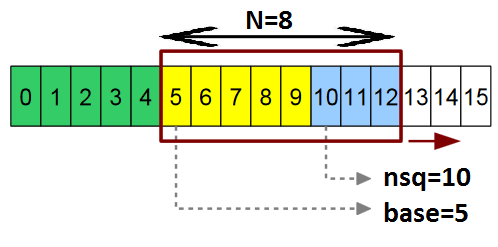
\includegraphics[scale=0.75]{window.png}\hss}\hfill\null
  \caption{Représentation d'une window. Le prochain paquet à être envoyé est celui de numéro 10}
\end{figure}

\subsection{"Two-way handshake"}
Commencer directement par l'envoi de paquets en pipelining engendrait des erreurs d'exécutions (seul le dernier paquet envoyé était reçu). Nous avons donc forcé le GbnSendingProtocol à commencer non pas par le paquet 0 mais par le paquet -1, et d'attendre la réception de l'ACK(-1) lui étant associé afin de commencer le pipelining. Le "two-way handshake" n'a pas été élargit jusqu'à un three-way handshake car nous n'en avons pas senti la nécéssité.

\subsection{Mise en oeuvre du Go-Back-N}
Le GbnSendingProtocol comporte trois méthodes majeures: \\
-\bfseries potentiallySend() \mdseries : Cette fonction enverra (récursivement) des paquets jusqu'à remplir la window (jusqu'à ce qu'nsq soit égal à base+N). Si aucun timer n'est en court, elle en lancera un, en focalisant l'attention du GbnSendingProtocol sur un paquet en particulier (stocké dans la varible int w) afin de pouvoir adapter plus tard le temps accordé par le timer avant un timeout \\
-\bfseries receive(source,datagram) \mdseries : Cette fonction, implémentation de la méthode receive de l'interface IPInterfaceListener, sera appelée lorsqu'un ACK sera reçu. Elle adaptera la window et le timer en conséquent. Si modification de la window a été fait (l'ACK confirme qu'un message a bien été reçu), elle se terminera pas l'appel de potentiallySend(). Si le controle de congestion est activé, elle s'occupera du cas potentiel d'ACK dupliqué. \\
-\bfseries timeOutReaction() \mdseries : Cette méthode sera appelée par le timer suite à un time out. Elle renvoit les messages de la window déjà envoyé (avant nsq), ces derniers n'ayant pas confirmé leurs réception (avec un ACK) assez rapidemment. (Ou simplement le paquet numéro -1 si le time out se produit lors du "two-way handshake").\\

Le GbnReceivingProtocol n'est composé que d'une fonction receive, envoyant théoriquement aux couches superieurs les données reçue si il s'agit bien des données attendues (l'affichant simplement dans cette implémentation) et un ACK dont le numéro de séquence sera celui du dernier paquet correctement reçu dans l'ordre (celui du paquet qui vient d'être reçu si il n'y a pas de problème)

Après avoir réalisé le "two-way handshake", le GbnSendingProtocol commencera donc le processus par un premier appel de potentiallySend(). \\ \\
On peut noter que le GbnSender garde tout les paquets à envoyer de sa sendingQueue même après envoi de ces derniers. Cela peut théoriquement poser problèmes si il y a beaucoup de données à envoyer et que le flux de nouveaux paquets à envoyer est plus ou moins continu. Il serrait bien entendu possible de corriger simplement cela en supprimant un paquet de la sendingQueue à chaque fois que l'ACK correspondant est reçu, décrémentant d'autant la valeur de nsq et de base en même temps.

\subsection{Adaptation du temps avant time-out}
Le temps accordé a un ACK pour être reçu suite à l'envoi d'un paquet, avant que le paquet soit considéré comme perdu et que le time-out soit déclenché, est régulièrement actualisé, et est stocké dans le GbnSendingProtocol de part la variable (de type int) tDeadLine. Le temps stocké dans tDeadLine est exprimé en millisecondes.\\
Initialement, tDeadLine prend la valeur arbitraire de 300, c'est à dire qu'une time out sera déclenché lors du premier envoi de paquet (celui du two-way handshake) après un temps de 300 ms.\\
tDeadLine est actualisé lors de la réception du paquet concerné par le timer, le paquet dont le numéro est celui de la variable w, auquel cas le temps d'envoi et réception du paquet est calculé puis multiplié par 2,5. La nouvelle valeur de tDeadLine est la moyenne entre son ancienne valeur et cette nouvelle valeur calculée. 
\[
   tDeadLine_{new} = \frac{tDeadLine_{old} + (PingPongTime * 2.5)}{2}
\]
Notons que, si aucun paquet n'est perdu et que le temps d'envoi d'un paquet/reception de son ACk ("PingPongTime") est constant, la valeur de tDeadLine va tendre vers ce temps multiplié par 2,5. \\
Si en revanche un time out se produit, la valeur de tDeadLine augmente de 10\%. Un garde-fou est également présent, se déclenchant si tDeadLine excède 5000ms, pour éviter de tourner en continu sur un réseau qui n'est visiblement plus fonctionnel.



\section{Contrôle de congestion}
Pour le contrôle de congestion nous avons décidé de faire en sorte que l'utilisateur puisse tout de suite choisir si celui-ci veut l'utiliser ou non dés le lancement de l'application. Si l'utilisateur décide de l'utiliser ce qui se passera c'est que le protocole d'envoi (\textbf{GbnSendingProtocol}) va initialiser la taille de la fenêtre \textbf{N} à 1. \\ 
Ensuite le programme va initier le \textit{goback-N} c'est-à-dire qu'il va lancer l'envoi de paquets avec tout d'abord une taille $N=1$ comme initialisé et lorsque notre \textbf{Sender} va recevoir le ACK correspondant au paquet envoyé il va appeler la méthode \textit{upgradeWindow()} qui va décider si l'on doit appliquer du "\textit{slow start}" ou de l'"\textit{additive increase}" en fonction de sa valeur par rapport au \textbf{ssthresh},le \textit{slow start threshold}, de la fenêtre (initalisé à la valeur $2^{32}-1$). Si notre N est strictement inférieur à \textbf{ssthresh} alors on applique la formule du \textit{slow start} qui dit : \[
\forall \text{ACK reçu correctement, }N_{new} = N_{old}+1 MSS.
\]\\
Sinon la méthode va utiliser de l'\textit{additive increase} à l'aide de la variable \textbf{current} qui est en fait la taille réelle de la fenêtre (qui est à la base une valeur entière). On le calcule comme suit:
\[
current_{new} = current_{old}+1/N 
\]
\[
si \ (int)\ current > N, alors \ N = current.
\]
\\
Si le \textbf{Sender} reçoit 3 ACKs dupliqués alors la méthode de réception va appliquer le \textit{multiplicative decrease} qui appliquera les changements suivants : 
\[
N_{new} = \begin{cases}
\frac{N_{old}}{2} & \text{si } N > 1 \\
1 & \text{sinon}
\end{cases}
\] 
\[
current = ssthresh = N_{new} 
\]\\
Enfin si le programme détecte un \textit{timeout} il effectuera les changements suivants :
\[
ssthresh = \begin{cases}
\frac{N_{old}}{2} & \text{si } N>1 \\
1 & \text{sinon}
\end{cases}
\]
\[
N_{new}=current = 1
\]
et par la suite effectuera le renvoi de paquets avec une taille de fenêtre de 1 et refera les différentes étapes de la congestion.\\
\end{document}
